% !TeX spellcheck = de_DE
\chapter{Friedmann-Gleichung\label{chapter:thema}}
\lhead{Friedmann-Gleichung}
\begin{refsection}
\chapterauthor{Andri Hartmann und Tobias Schuler}
\printbibliography[heading=subbibliography]
\lhead{Einleitung zur Friedmann-Gleichung}
\rhead{}
\begin{quote}
	\textit{Wir dürfen das Weltall nicht einengen, um es den Grenzen unseres Vorstellungsvermögens anzupassen, wie der Mensch es bisher zu tun pflegte. Wir müssen vielmehr unser Wissen ausdehnen, sodass es das Bild des Weltalls zu fassen vermag.}\footnote{Sir Francis von Verulam Bacon (1561 - 1626)}
\end{quote}
In diesem Kapitel möchten wir euch helfen, gemäss dem oben erwähnten Zitat, das Bild des Weltalls fassen zu vermögen. Um dies zu tun, werden wir versuchen, das Gebilde, welches wir Universum nennen, unter Zuhilfenahme der physikalischen Gesetze in einen mathematischen Kontext zu bringen.

\section{Vorgeschichte}
Mit der Formulierung der Allgemeinen Relativitätstheorie durch Albert Einstein war es erstmals möglich,
sich seriös Gedanken über die Geschichte des
Universums zu machen. An dieses Problem haben sich anfangs der 20er Jahre bekannte Wissenschaftler wie Einstein, deSitter, Friedmann und Lemaitre gemacht. 
Zu dieser Zeit gab es wenig bis keine experimentellen Daten, die Aussagen über Geometrie oder Dynamik des Weltalls hätten treffen können. So kam es, das unter den führenden Astronomen das Bild eines statischen Universums grosse Empathie erhielt.

Durch die Entdeckung der Fluchtbewegungen von Galaxien mithilfe der kosmologischen Rotverschiebungen gelang es 1929 dem US-amerikanischen Astronomen Edwin Hubble, die damalige Vorstellung eines statischen Kosmos zu widerlegen. Diese Entdeckung hatte zur Folge, dass man jetzt ein Modell mit einem sich veränderndem Weltradius brauchte.
\pagebreak
\section{Skalenfaktor a\label{Section:Skalenfaktor}}
Um ein dynamisches Universum beschreiben zu können, führen wir ein dreidimensionales Koordinatensystem ein, welches sich mit der relativen Bewegung von Galaxien mitbewegen kann. In einem solchen System besitzen die Objekte fixe Koordinaten und sind somit wie in einem Raster eingefroren. Die Einheit des Rasters wird durch den {\em Skalenfaktor} $a$ ausgedrückt und ist eine Funktion der Zeit. Ein zweidimensionales Raster ist in Abbildung \ref{friedmann:friedmannRaster} zu sehen. Die drei Kreise stellen Galaxien dar. Die Linie zwischen der roten und blauen Galaxie zeigt den Abstand. Dehnt sich nun das Universum aus, dehnt sich das Raster mit, wie auf dem zweiten Plot zu sehen ist. Die Grösse der Galaxien und die Position auf dem Raster bleiben gleich, der Abstand zwischen den Galaxien hat sich aber verändert. 

\begin{figure}[h]
	\centering
	\includegraphics[width  = \textwidth]{friedmann/images/rasterFriedmann.pdf}
	\caption{Raster ums Universum für zwei verschiedene Skalenfaktoren}
	\label{friedmann:friedmannRaster}
\end{figure}%
\subsection{Mathematische Beziehungen im Koordinatensystem \label{friedmann:Beziehungen im Koordinatensystem}}
Die Distanz zwischen zwei Punkten A und B entspricht 
\begin{equation}
D_{AB}(t)\, = \sqrt{a^2(t)\Delta_{AB}\,x^2 + a^2(t)\Delta_{AB}\,y^2 + a^2(t)\Delta_{AB}\,z^2}\, =\, a(t) \sqrt{\Delta_{AB}\,x^2 + \Delta_{AB}\,y^2 + \Delta_{AB}\,z^2}
\label{friedmann:Abstand}
\end{equation}
F\"{u}r die Geschwindigkeit, mit der sich die beiden Punkte relativ zueinander bewegen, gilt 
\begin{equation}
v_{AB}(t) = \dfrac{dD_{ab}}{dt} 
= \dot{a}(t) \sqrt{\Delta_{AB}\,x^2 + \Delta_{AB}\,y^2 + \Delta_{AB}\,z^2}
\label{friedmann:geschwindigkeit}
\end{equation}
Um nun Aussagen über die Dynamik des Universums zu machen, die nicht von der fiktiven Wahl des Skalenfaktors abhängen, teilen wir die Geschwindigkeit durch den Skalenfaktor $a$.
\begin{equation}
\frac{v_{AB} }{D_{AB}} = \frac{\dot{a}}{a}
\end{equation}
%\begin{satz} [Hubble-Konstante]
%	Die Ableitung des Skalenfaktors dividiert durch den Skalenfaktor entspricht der Hubble-Konstante.
%	\[
%	\frac{\dot{a}}{a} = H
%	\]
%\end{satz}
\begin{satz}[Kosmologisches Prinzip]
\label{Prinzip:kosmologisches Prinzip}
Das kosmologische Prinzip besagt, dass auf einer grossen Längenskala kein Ort im Universum gegenüber einem anderen ausgezeichnet ist. Diese Annahme bedingt zwei Eigenschaften, Isotropie und Homogenität. Isotropie  bezeichnet die Unabhängigkeit einer Eigenschaft von der Richtung, Homogenität die Gleichheit einer physikalischen Eigenschaft über die gesamte Ausdehnung eines Systems.
\end{satz}
Gemäss Satz (\ref{Prinzip:kosmologisches Prinzip}) und der Eigenschaft unseres Koordinatensystems, Kap.(\ref{Section:Skalenfaktor}), bleibt die Masse in einem Einheitskubik konstant über die Zeit. Somit ist die Masse $M$ in einem Würfel mit Dimension $\Delta x$, $\Delta y$ und $\Delta z$ 
\begin{equation}
M_{xyz} = \mu \,\Delta x \,\Delta y \,\Delta z
\end{equation}
Der Parameter $\mu$ beschreibt die Massendichte in einem Einheitsquadrant und ist somit von der Wahl von $a$ abhängig, jedoch konstant über die Zeit. Das Volumen des Würfels ist bekanntlich
\begin{equation}
V_{xyz} = a^3 \,\Delta x \,\Delta y \,\Delta z
\end{equation}
und folglich kann die Massendichte geschrieben werden als
\begin{equation}
\rho = \frac{M_{xyz}}{V_{xyz}} = \frac{\mu}{a^3}
\label{friedmann:dichte}
\end{equation}
Es stellt sich nun die spannende Frage: Wie ändert sich der Skalenfaktor mit der Zeit? Und eben diese Frage wird mit der Friedmann-Lema\^{i}tre Differentialgleichung beantwortet.

\section{Alexander Friedmann und Georges Lema\^{i}tre}
Die sogenannte Friedmann-Lema\^{i}tre-Gleichung beschreibt das Verhalten des Universums nach der Inflation des Kosmos im Rahmen des Standard-Urknall-Modells. Die {\em Energiedichte} $\rho$, die {\em Krümmung} $\kappa$ und die {\em kosmologische Konstante} $\Lambda$ sind die Parameter der Gleichung.
\begin{equation}
\left(\frac{\dot{a}}{a}\right) ^2 = \frac{8 \pi G}{3} \rho - \frac{\kappa c^2}{a^2} + \frac{\Lambda c^2}{3}
\end{equation}
Bevor wir beginnen, die Gleichung herzuleiten, können wir schon jetzt verschiedene Lösungen für unterschiedliche Parameterwerte diskutieren. Das hilft uns später beim Rekonstruieren der Geschichte des Universums.

\subsection{Masseloses Universum \label{friedmann:masselosesUniversum}}
%Sie könnten zum Beispiel könnten zum Beispiel mit einem leeren Universum beginnen (rho = 0), und die Gleichung einfach mal für den zweiten und dritten Term lösen. Rein mathematisch, ohne die Physik schon zu untersuchen. Hier können Sie den Trick mit der zusätzlichen Ableitung?? erklären. Damit zeigen Sie schon mal, dass die Gleichung eine Vielzahl spannender Lösungen hat.
Setzen wir $\rho = 0$, entspricht dies einem masselosen Universum.  Wir schreiben die Gleichung ohne den ersten Term
\[\left(\frac{\dot{a}}{a}\right) ^2 = - \frac{\kappa c^2}{a^2} + \frac{\Lambda c^2}{3}\]
Nun sind noch zwei Terme übrig. Separiert man sie, findet man eine Lösung wie folgt
\begin{enumerate}
	\item $\kappa = 0$ 
		\begin{align}
			\nonumber \left(\frac{\dot{a}}{a}\right) ^2 &= \frac{\Lambda c^2}{3}  &&| \cdot a^2 \\
			\nonumber \dot{a} ^2 &= \frac{\Lambda c^2 a^2}{3}  &&|\sqrt{...}\\
			\nonumber \dot{a} &= \sqrt{\frac{\Lambda c^2}{3}} a &&|\sqrt{\frac{\Lambda c^2}{3}} := E \ge 0 \, (!)\\
			\nonumber \dot{a} &= E \cdot a &&|\int ...\, dt \\
			a &= e^{E \cdot t} \label{friedmann:Lambda}
		\end{align}
	
	
Mit $\kappa = 0$ gibt es zwei mögliche Ausprägungen für das Universum, entweder ist $E = 0$ oder $E > 0$. Im ersten Fall wäre das Universum statisch und wäre für alle Zeit gerade so gross wie der Skalenfaktor. Im zweiten Fall würde sich das Universum exponentiell ausdehnen.


		
	\item $\Lambda = 0$ 
		\begin{align}
			\nonumber \left(\frac{\dot{a}}{a}\right) ^2 &= - \frac{\kappa c^2}{a^2}  \qquad &&| \cdot a^2\\
			\nonumber \dot{a} ^2 &= - \kappa \, c^2 \qquad &&|\sqrt{...}\\
			\nonumber \dot{a} &= \sqrt{- \kappa}\, c \qquad &&|\int ...\, dt \\
			a &= \sqrt{- \kappa}\, c \cdot t \label{friedmann:Kappa}
		\end{align}
		
Auch hier gibt es zwei mögliche Ausprägungen. Wie vorhin könnte $\kappa = 0$ sein, oder $\kappa < 0$. In diesem Fall würde das bedeuten, es entsteht entweder kein Raum, da der Skalenfaktor $a$ nie anwächst, oder aber das Universum wächst linear mit der Zeit an.
	
\end{enumerate}

\subsection{Universum mit Masse \label{friedmann:UniversumMitMasse}} 
Wie vorher schon angedeutet, steht $\rho$ für die Dichte des Universums. Ist das Universum masselos, ist die Dichte null. Gehen wir aber davon aus, dass im Universum Materie vorhanden ist, findet man eine weitere Lösung der Differentialgleichung. Zu beachten ist, dass die Dichte abhängig von der Ausdehnung ist. Als Gedankenstütze kann man sich eine geschlossene Box gefüllt mit einem homogenen Gas vorstellen. Vergrössert sich die Box nun wie sich das Universum ausdehnt, nimmt die Dichte ab solange kein Gas hinzugefügt wird. Dies ist auch in Abbildung (\ref{friedmann:friedmannRaster}) zu sehen. Das Raster ist im zweiten Plot grösser geworden, die Masse im Raster hat aber nicht zugenommen. Die Ausdehnung geschieht in einem dreidimensionalen System kubisch, die Massendichte muss also kubisch abnehmen. Damit die Gleichung lösbar ist, vernachlässigen wir den $\Lambda$- und $\kappa$-Term. Für die Dichte setzen wir (\ref{friedmann:dichte}) ein. 
\[\left(\frac{\dot{a}}{a}\right) ^2 = \frac{8 \pi G}{3} \frac{\mu}{a^3}\]
Weiter können wir $\mu$ so wählen, dass sich der konstante Term als eins schreiben lässt.
\[\left(\frac{\dot{a}}{a}\right) ^2 = \frac{1}{a^3}\]
Um die Gleichung zu lösen, ziehen wir die Quadratwurzel und multiplizieren mit $a$.
\begin{align}
	\nonumber \dot{a} &= \frac{1}{\sqrt{a}} \\
	\nonumber \frac{da}{dt} &=\frac{1}{\sqrt{a}} \\
	\nonumber \frac{dt}{da} &= \sqrt{a} \\
	\nonumber t &= \frac{2}{3} a^{3/2} \\
	a &= \frac{3}{2} t^{2/3} \label{friedmann:Masse}
\end{align}

\subsection*{Diskussion der Lösungen}
Wir finden also für jeden Term in der Gleichung eine andere Beschreibung der Bewegung des Universums. Betrachten wir die Anfangsgleichung genauer, können wir herauslesen, welcher Term bei einer gegebenen Grösse $a$ dominiert.
\begin{align*}
\left(\frac{\dot{a}}{a}\right) ^2 =\;\frac{8 \pi G}{3} \rho\; &- \;\frac{\kappa c^2}{a^2}\; + \;\frac{\Lambda c^2}{3} \\
\left(\frac{\dot{a}}{a}\right) ^2 = \;\frac{8 \pi G}{3} \frac{\mu}{a^3}\; &-\;\frac{\kappa c^2}{a^2}\; +\; \frac{\Lambda c^2}{3}
\end{align*}
Für kleine Werte von $a$ wird der erste Term dominieren, für mittlere Werte von $a$ der Zweite, und für grosse Werte dominiert der letzte Term. Das heisst, die Lösungen setzen sich in zeitlicher Reihenfolge wie folgt zusammen:
Gleichung (\ref{friedmann:Masse})  dominiert zu Beginn, dann mischt sich Gleichung (\ref{friedmann:Kappa}) ins Spiel, und am Schluss dominiert Gleichung (\ref{friedmann:Lambda}) über das Schicksal des Universums. In Abbildung (\ref{friedmann:mathematischFriedmann}) ist die numerische Lösung der Differentialgleichung mit allen Termen eingezeichnet.
Zu bemerken ist, dass die Abbildung in erster Linie als qualitative Anschauung zu betrachten ist, da wir die Parameter zur einfacheren Betrachtung angepasst haben. Ohnehin führen diese Anpassungen aber nicht zu einer falschen Vorstellung der Bedeutsamkeit der Terme, da diese nur die Vorfaktoren, nicht aber die Potenzen beeinflussen. 
\footnote{Für $\kappa$ wurde eine negative Zahl eingesetzt. Der Fall $\kappa = 0$ vernachlässigen wir, da die Lösung nur aus (\ref{friedmann:Masse}) und (\ref{friedmann:Lambda}) besteht.}
\begin{figure}[h]
	\centering
	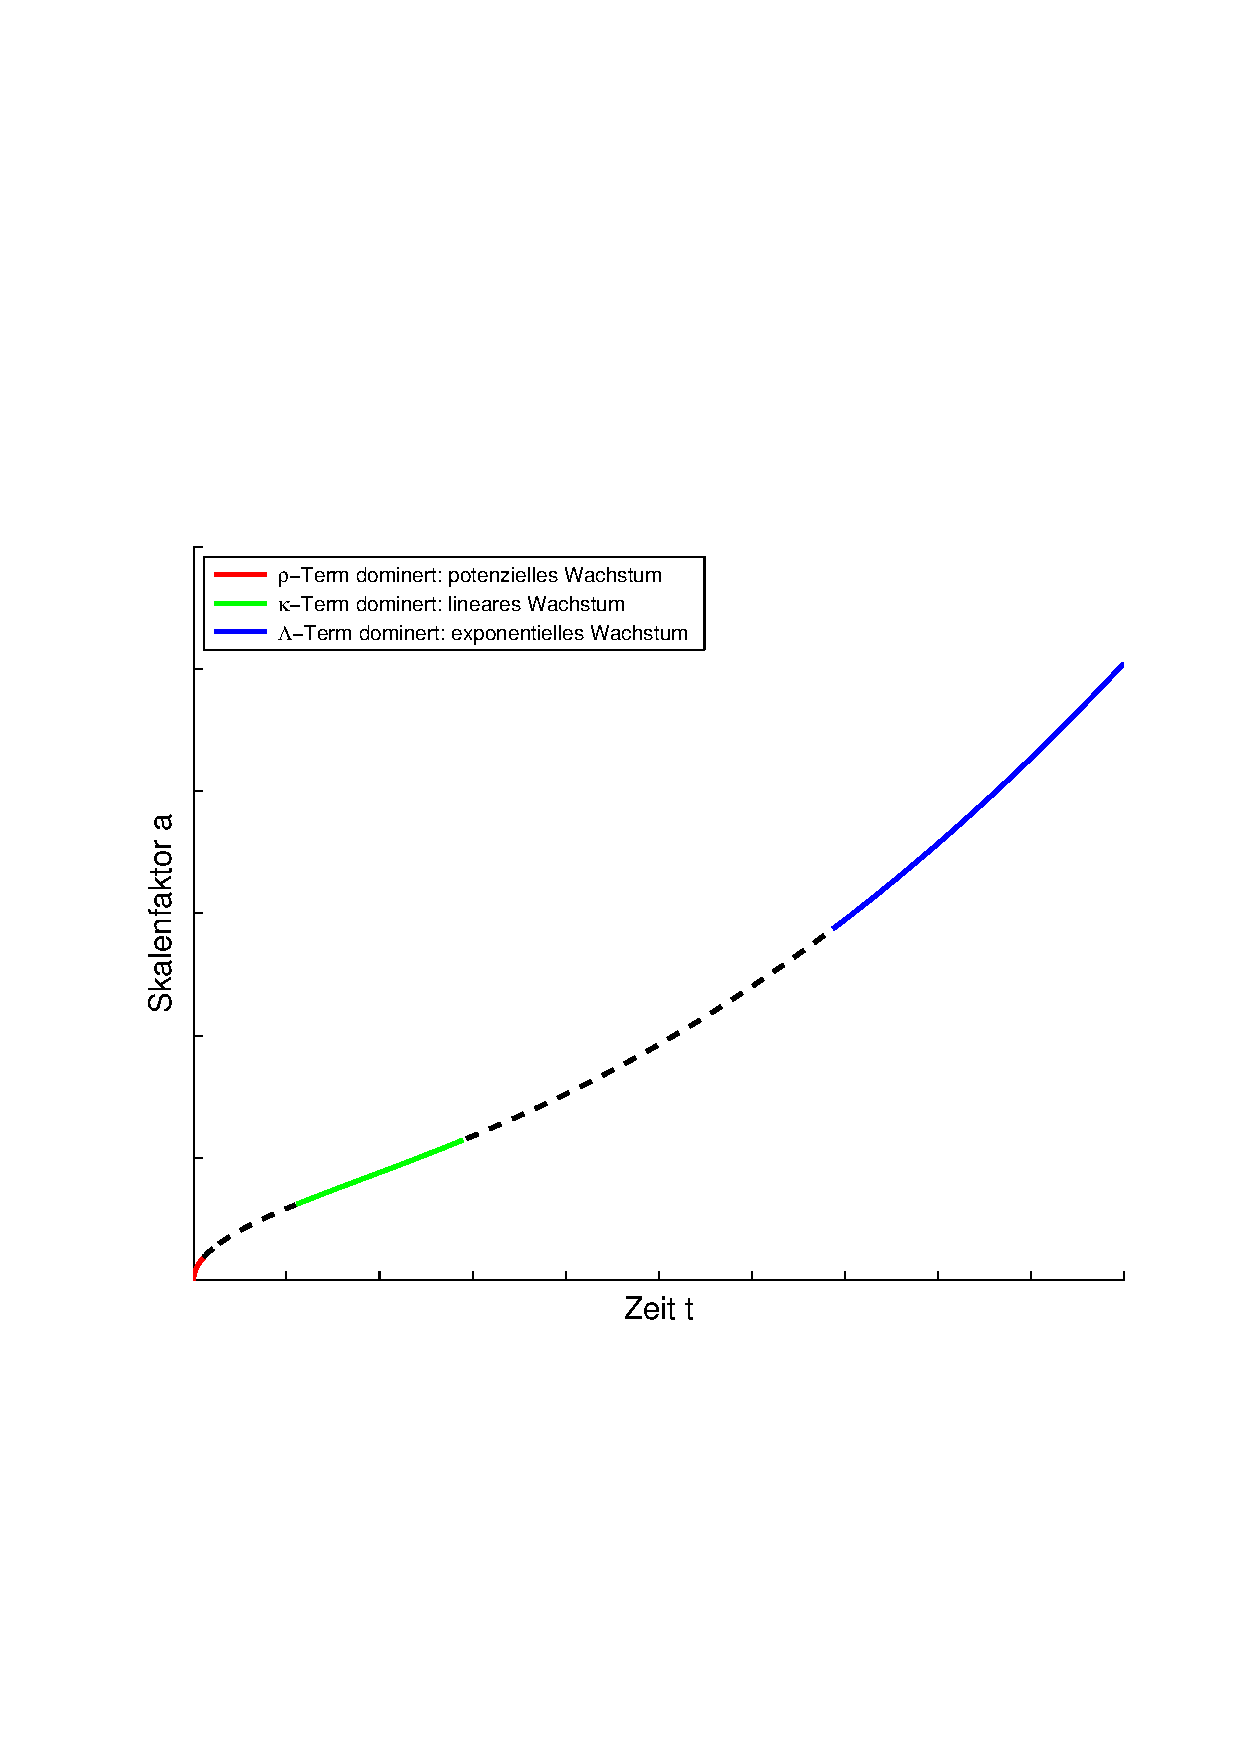
\includegraphics[width = 0.8\textwidth]{friedmann/images/mathematischFriedmann.pdf}
	\caption{Mathematische Bedeutung für die Ausbreitung des Universums der einzelnen Terme}
	\label{friedmann:mathematischFriedmann}
\end{figure}%
\subsection{Herleitung der Differentialgleichung}
Im folgenden Abschnitt versuchen wir die Bedeutung der einzelnen Terme physikalisch zu hinterlegen. Das ist nicht immer ganz einfach, denn die Differentialgleichung wurde unter anderem mithilfe der Einsteinschen Feldgleichungen hergeleitet worden. In diesem Kapitel werden wir aber nicht so weit gehen, trotzdem können wir einige interessante Relationen mithilfe der klassischen Physik herleiten.
\subsubsection{Newtonscher Ansatz}
Um die relative Beschleunigung zweier Punkte im Universum zu beschreiben, wird von folgendem Ansatz ausgegangen: Ein Beobachter befindet sich im Ursprung des Koordinatensystems und ist in Ruhe. Um nun die Kraft auf einen Körper der {\em Masse} $m$ im {\em Abstand} $D$ zu berechnen, denkt man sich eine Kugelschale um den Ursprung mit {\em Radius} $D$. Die Kraft auf den Körper verhält sich wie die Punktmasse aller  einzelnen Körper in der Kugel im Ursprung gedacht.
Im folgenden Abschnitt werden die in Kap.(\ref{friedmann:Beziehungen im Koordinatensystem}) hergeleiteten Formeln angewendet. Einfachheitshalber schreiben wir für den Abstand im Grid
\[ \sqrt{\Delta x^2 + \Delta y^2 + \Delta z^2} := R \]
und für das Volumen V der Kugel
\[V_\text{Kugel} = \frac{4 \pi }{3} a^3 R^3\]
Gemäss Newton ergibt sich die Gravitationskraft aus
\begin{equation}
F_G = -\frac{m M G}{D^2}
\end{equation}
Da die Gravitationskraft zwecks Vereinfachung des Modells als einzige Kraft eingesehen wird, gilt für die Beschleunigung mit 
\[F = m A\]
\[A = - \frac{M G}{D^2} = \ddot{a} R \quad\Leftrightarrow\quad \ddot{a} = \frac{- M G}{a^2 R^3} \quad\Leftrightarrow\quad \frac{\ddot{a}}{a} = \frac{-\frac{4 \pi }{3} M G}{\frac{4 \pi}{3}a^3 R^3} \quad\Leftrightarrow\quad \frac{\ddot{a}}{a} = \frac{- 4 \pi G}{3} \frac{M}{V_\text{Kugel}}\]
Die Gleichung wurde so angepasst, dass oben die Masse und unten das Volumen steht. Damit vereinfacht sich die Beschleunigung zu
\begin{equation}
\frac{\ddot{a}}{a} = \frac{- 4 \pi G}{3} \rho
\end{equation}
\subsubsection{Bedeutung der Beschleunigungsgleichung}
Setzt man für die Dichte Gleichung (\ref{friedmann:dichte}) ein ergibt sich
\[\frac{\ddot{a}}{a} = \frac{- 4 \pi G}{3} \frac{\mu}{a^3} \]
Durch geschickte Wahl des Skalenfaktors kann $\mu$ den konstanten Term auf der rechten Seite gegen 1 streben lassen. So vereinfacht sich die Gleichung zu
\[\frac{\ddot{a}}{a} = \frac{-1}{a^3} \qquad\Leftrightarrow\qquad \ddot{a} = \frac{-1}{a^2}\]
Die Differentialgleichung ist nichtlinear  und nicht lösbar. Trotzdem können wir gewisse Aussagen machen, nämlich
\begin{enumerate}
	\item Die negative Beschleunigung wirkt der Ausdehnung des Universums entgegen. 
	\item Statisches Universum ist nicht möglich für $\rho \neq 0$.
	\item Die Formel hängt nicht vom Ort $R$ ab, was bedeutet das unser Ansatz mit dem Beobachter im Ursprung legitim war.
\end{enumerate}

\subsubsection{Energieerhaltung}
Da wir versuchen, das Universum als ein physikalisches System zu beschreiben, muss auch hier der bedeutsame Satz der Energieerhaltung gelten. Im folgenden befassen wir uns mit der radialen Ausdehnung des Universums aus einem Ursprung heraus (Big Bang). Das Universum kann bei der Entstehung mit verschiedenen Gesamtenergien initialisiert werden, abhängig von der Dichte der Materie und ihrer Fluchtgeschwindigkeit. Betrachten wir für den Anfang die Beziehung zwischen kinetischer und potentieller Energie.
\begin{equation}
E_{\text{ges}} = E_{\text{kin}} - E_{\text{pot}} =  \frac{m v^2}{2} - \frac{m M G }{D}, \qquad D = \text{Abstand zwischen der Masse M und m}
\end{equation}
Wir werden später noch andere Formen von Energie kennenlernen, die wir dieser Gleichung hinzufügen müssen. Doch beginnen wir in kleinen Schritten. Die Gesamtenergie kann nun drei wesentliche, für die Dynamik interessante Werte annehmen, nämlich
\begin{enumerate}
	\item $E_{ges} > 0 \rightarrow$ Eine Masse $m$ entflieht der Schwerkraft.
	\item $E_{ges} = 0 \rightarrow$ Eine Masse $m$ nähert sich asymptotisch  der Geschwindigkeit null, bleibt aber nie stehen. (Fluchtgeschwindigkeit)
	\item $E_{ges} < 0 \rightarrow$ Eine Masse $m$ wird so stark angezogen, dass die Geschwindigkeit ihre Richtung ändert.
\end{enumerate}
Nennen wir die Gesamtenergie eine Konstante $E$ und formen die Gleichung um.

\begin{align*}
	\frac{m v^2}{2} - \frac{m M G}{x} &= E_1 &&| \cdot\frac{2}{m} \\ 
	v^2 - \frac{2 M G}{x} &= \frac{2E_1}{m} = E_2\\	
\end{align*}
Wir setzen (\ref{friedmann:geschwindigkeit}) und (\ref{friedmann:Abstand}) ein.
\begin{align*}
	\left( \dot{a} \, R\right)^2 &= \frac{2 M G}{a\,R} + E_2 &&| \cdot \frac{1}{a^2\,R^2}\\
	\frac{\dot{a}^2}{a^2} &= \frac{2 M G}{a^3 R^3} + \frac{E_2}{a^2 R^2} \\
	\left(\frac{\dot{a}}{a} \right)^2 &= \frac{\frac{4 \pi}{3}2 M G}{\frac{4 \pi}{3} a^3 R^3} + \frac{E_2}{a^2 R^2}
\end{align*}
Auf der rechten Seite der Gleichung erscheint jetzt die Masse der Kugel mit Radius $R$ dividiert durch das Kugelvolumen $V$, was der Dichte entspricht. Daraus resultiert die vereinfachte Differentialgleichung 
\begin{equation}
\left(\frac{\dot{a}}{a} \right)^2 = \frac{8 \pi G}{3} \rho + \frac{E_2}{a^2 R^2}
\label{friedmann:EnergieerhaltungUniversum}
\end{equation}
Mit (\ref{friedmann:dichte})
\[\left(\frac{\dot{a}}{a} \right)^2 = \frac{8 \pi G}{3} \frac{\mu}{a^3} + \frac{E_2}{a^2 R^2} \\\]
Wir wählen die Konstanten $\mu$ und $R$ so, dass die Gleichung folgendermassen vereinfacht wird:
\begin{equation}
\left(\frac{\dot{a}}{a} \right)^2 = \frac{1}{a^3} + \frac{E}{a^2}
\end{equation}

\subsubsection{Diskussion der Differentialgleichung}
Wir erinnern uns, die Konstante $E$ steht für die Gesamtenergie des Universums und kann positiv, negativ oder null sein.
\begin{enumerate}
	\item Beginnen wir mit dem einfachsten Fall und setzen $E = 0$.
	\[\left(\frac{\dot{a}}{a} \right)^2 = \frac{1}{a^3}\]
	Diese Gleichung wurde im Kapitel (\ref{friedmann:UniversumMitMasse}) schon gelöst. Ist die Gesamtenergie $E$ null, dehnt sich das Universum gemäss Gleichung (\ref{friedmann:Masse}) aus. Je grösser also das Universum wird, desto kleiner wird die Geschwindigkeit der Ausdehnung.
	\[\lim_{t\to\infty} \dot{a}(t) = 0\]
	\item Für den zweiten Fall ist $E > 0$.
	\[\ \left(\frac{\dot{a}}{a} \right)^2 = \frac{1}{a^3} + \frac{E}{a^2}\]
	Betrachten wir die rechte Seite, bemerken wir den Potenzunterschied im Nenner. Daraus folgt, dass für {\em kleine} $a$'s der {\em erste} Term dominiert, während der {\em zweite} Term für {\em grosse} $a$'s dominiert. Das kleine Universum verhält sich also wie für $E = 0$. Das grosse Universum hingegen verhält sich wie das massenlose Universum in (\ref{friedmann:masselosesUniversum}) mit $\Lambda = 0$.  
	
	\item Als letztes soll $E < 0$ sein
	\[\ \left(\frac{\dot{a}}{a} \right)^2 = \frac{1}{a^3} - \frac{|E|}{a^2} \qquad \Leftrightarrow \qquad \dot{a}^2 = \frac{1}{a} - |E|\]
	\begin{equation}
	\dot{a} = \pm \sqrt{\frac{1}{a} - |E|}
	\end{equation}
	Anhand des Phasendiagramms \ref{friedmann:phasenportrait} erkennt man die Lösung der drei Fälle. Solange $E \geq 0$ ist, dehnt sich das Universum unbeschränkt aus. Ist $E < 0$ dehnt sich das Universum bis zu einem gewissen Punkt aus. An diesem Punkt ist die Ausdehnungsgeschwindigkeit null. Danach beschreibt die Kurve ein in sich zusammenfallendes Universum, auch Big-Crunch genannt.
	
\end{enumerate}

\begin{figure}[h]
	\centering
	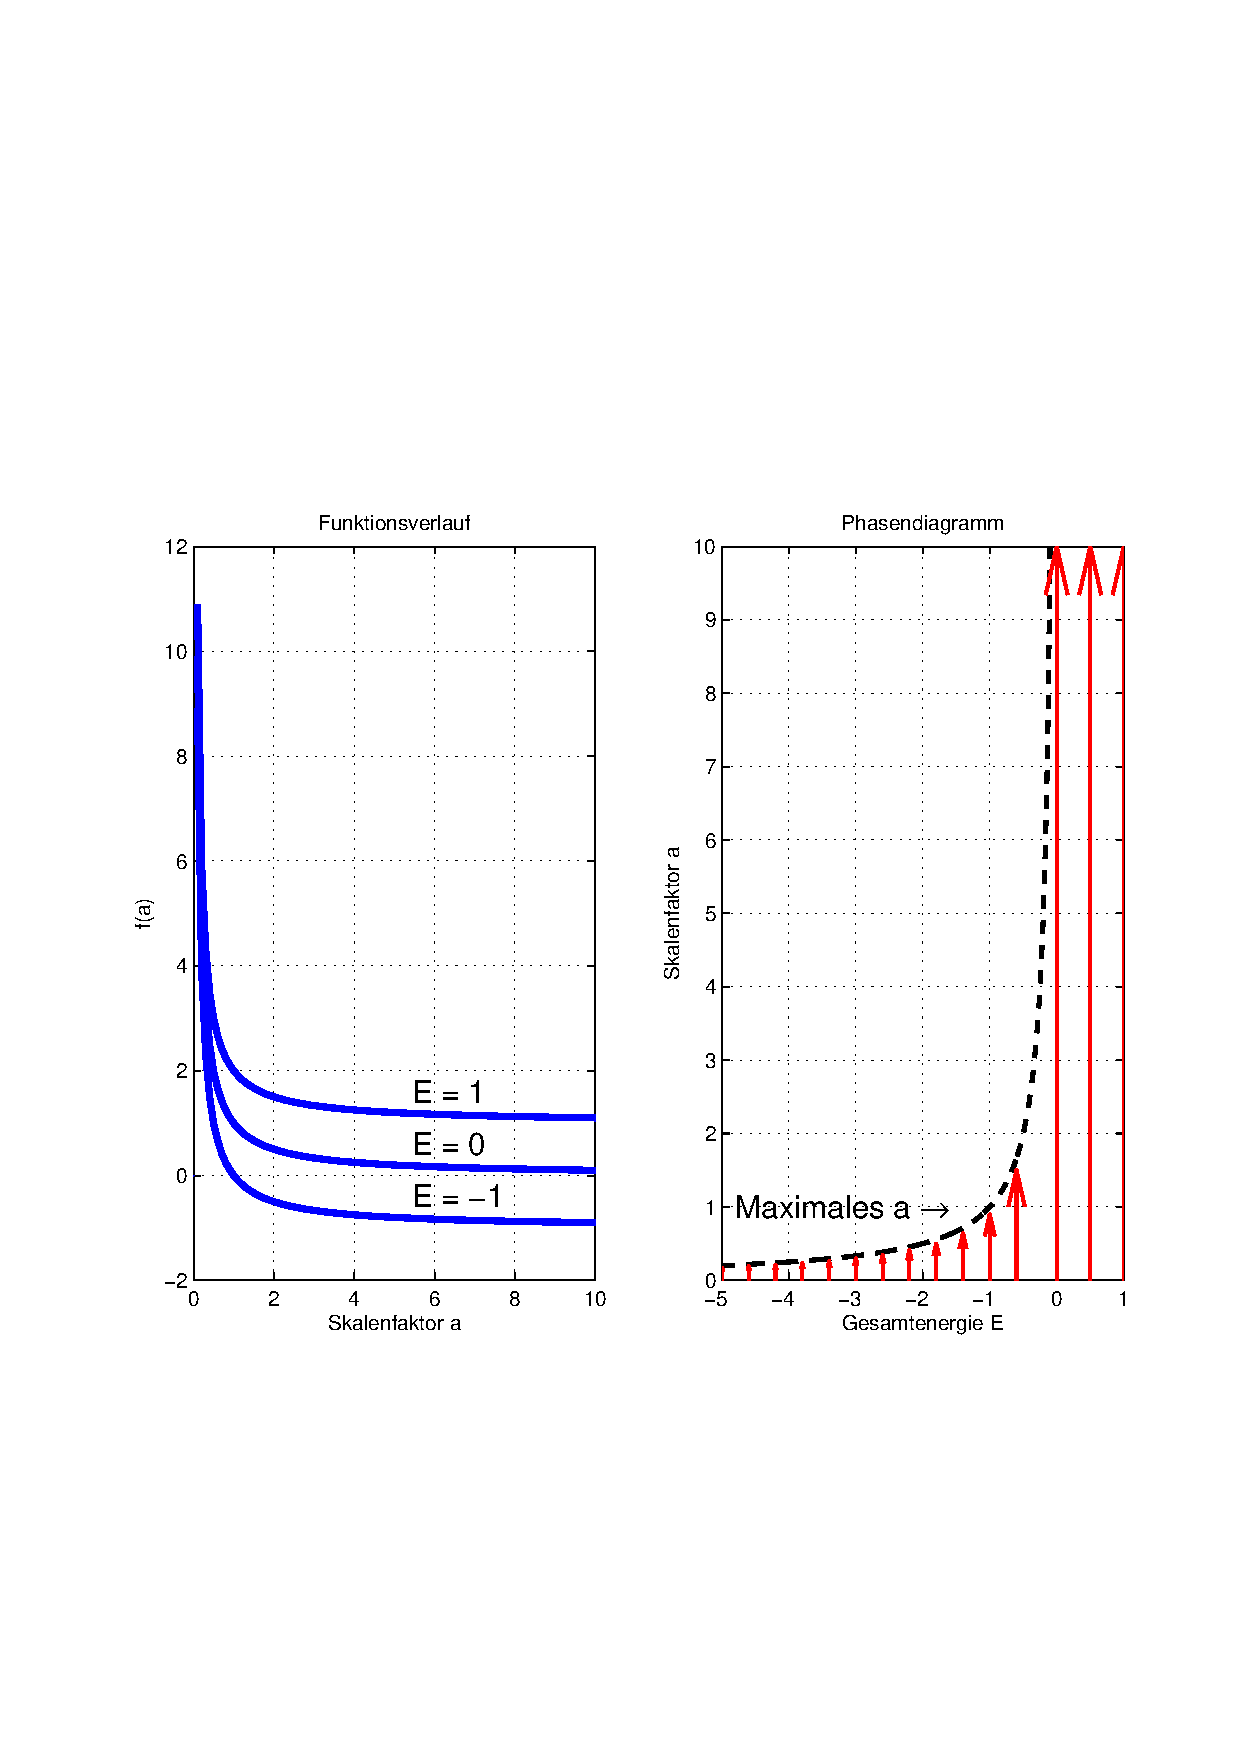
\includegraphics[width  = \textwidth]{friedmann/images/phasendiagramm.pdf}
	\caption{Phasenportrait in Abhängigkeit der Gesamtenergie c
		\label{friedmann:phasenportrait}}
\end{figure}%

\subsection*{Energiedichte}
Wie wir wissen, existiert im Weltall nicht nur sichtbare, sondern auch dunkle Materie und Strahlung. Dunkle Materie verhält sich in Bezug auf die gravitative Wirkung ähnlich wie sichtbare Materie, und deshalb wird im Folgenden nicht weiter darauf eingegangen.
Anders verhält es sich mit der kosmischen Strahlung in Bezug auf die Dynamik des Kosmos. Wir schreiben
\[ E_{str} = \frac{h c}{\lambda} \]
wobei $h$ die {\em Planksche Konstante}, $c$ die {\em Lichtgeschwindigkeit} und $\lambda$ die {\em Wellenlänge} des Photons ist.
Nun ist die Energie der Strahlung (z.B. eines Photons) in einem sich ausdehnenden Universum nicht konstant, sondern ändert sich mit der Zeit. 
Denn, vergrössert sich die Raumzeit während der Laufzeit um einen Faktor n, so geschieht dies auch mit der Wellenlänge des Strahls. Das bedeutet, dass die Energie eines Photons umgekehrt proportional zum Skalenfaktor $a$ ist. Für die Energiedichte der Strahlung bedeutet dies, dass sie sich nicht nur kubisch wie bei der baryonischen Materie ändert, sondern mit vierter Potenz.
\begin{equation}
\rho_{str} = \frac{\mu_{\text{str}}}{a^4}
\end{equation}
In die Gleichung der Energieerhaltung des Universums (\ref{friedmann:EnergieerhaltungUniversum}) setzen wir $\rho_{str}$ ein.
\[\left(\frac{\dot{a}}{a} \right)^2 = \frac{8 \pi G}{3} \frac{\mu_{\text{str}}}{a^4} + \frac{E_2}{a^2 R^2}\]
Wir wählen die Konstanten $\mu_{\text{str}}$ und $R$ so, dass die Gleichung vereinfacht wird zu
\[\left(\frac{\dot{a}}{a} \right)^2 = \frac{1}{a^4} + \frac{E}{a^2} \Leftrightarrow \dot{a} = \sqrt{\frac{1}{a^2} + E}\]
Wiederum ist die Differentialgleichung nicht elementar lösbar. Trotzdem können wir sagen, dass für {\em kleine} $a$'s der erste Term dominiert, während der zweite Term für {\em grosse} $a$'s dominiert. Setzen wir die Gesamtenergie des Universums $E$ gleich null, findet sich die neue Gleichung für den dominierenden erster Term.	
\[\left(\frac{\dot{a}}{a} \right)^2 = \frac{1}{a^4}\]
Um die Gleichung zu lösen, ziehen wir die Quadratwurzel und multiplizieren mit $a$.
\begin{align}
	\nonumber\dot{a} &= \frac{1}{a} \\
	\nonumber\frac{da}{dt} &=\frac{1}{a} \\
	\nonumber\frac{dt}{da} &= a\\
	\nonumber t &= \frac{1}{2} a^{2}\\
	a &= \sqrt{2}\,t^{1/2} 
\end{align}
Analog zum Newtonschen Ansatz verhält sich das Universum für einen dominierenden zweiten Term gemäss Gleichung (\ref{friedmann:Kappa}). 
Im Vergleich mit dem Universum, bei der die gewöhnliche Materie dominiert, ist vor allem zu Beginn ein Unterschied auszumachen. Die Strahlung lässt das Universum am Anfang viel schneller expandieren, siehe Abb. (\ref{friedmann:strahlungMaterie}) 

\begin{figure}[h]
	\centering
	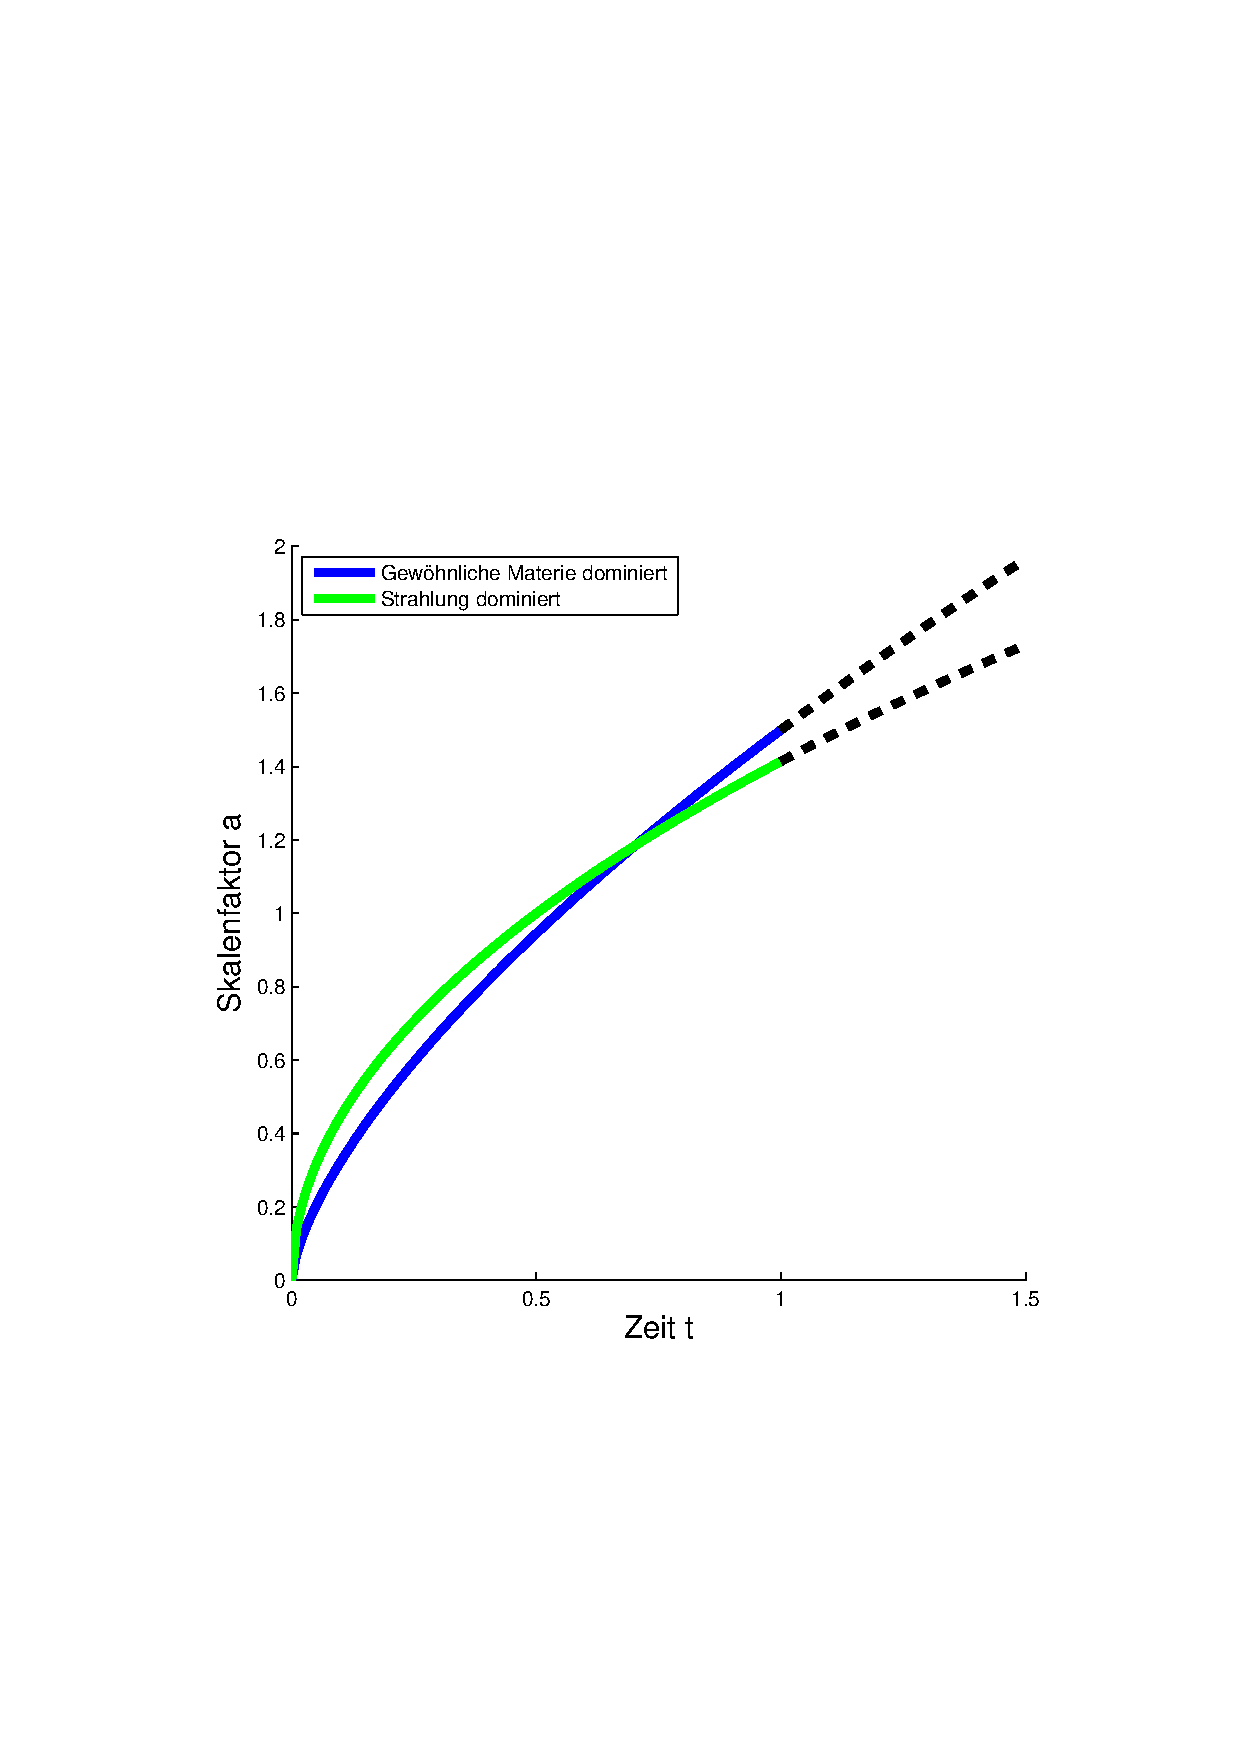
\includegraphics[width  = 0.8\textwidth]{friedmann/images/strahlungMaterie.pdf}
	\caption{Strahlung und Materie im Vergleich
		\label{friedmann:strahlungMaterie}}
\end{figure}

\subsection{Geometrie des Raumes}
Die bisher gemachten Überlegungen berücksichtigen nur die klassische oder newtonsche Physik, tatsächlich spielen die relativistischen Gesetze Einsteins eine wesentliche Rolle bei der Beschreibung des Universums. Einsteins Gesetze ändern die Gleichung (\ref{friedmann:EnergieerhaltungUniversum}) folgendermassen:  
\begin{equation}
	\left(\frac{\dot{a}}{a}\right) ^2 = \;\frac{8 \pi G}{3} \rho \; -\;\frac{\kappa c^2}{a^2}
\end{equation}
Der $\kappa$-Parameter beschreibt die Krümmung des Raumes (\ref{friedmann:GeometrieDesRaumes}).\footnote{Die Krümmung des Raumes kann durch Messen von Winkelsummen im Dreieck bestimmt werden.}  
\begin{table}[h]
\centering
\begin{tabular}{|>{$}r<{$}|>{$}r<{$}|>{$}c<{$}|}
\hline
\kappa&\text{Geometrie}&\text{Winkelsumme}\: \Delta\\
\hline
+1 & \text{Elliptisch} & > 180^\circ\\
0  & \text{Euklidisch} & =180^\circ\\
-1 & \text{Hyperbolisch} & <180^\circ\\
\hline	
\end{tabular}
\caption{Bedeutung von $\kappa$ für die Geometrie des Raumes\label{friedmann:GeometrieDesRaumes}}
\end{table}
Mathematisch gesehen hat der $\kappa$-Term abgesehen vom Vorzeichen die gleiche Bedeutung wie die Gesamtenergie des Universums,die im Kapitel \ref{friedmann:EnergieerhaltungUniversum} behandelt wurde, nämlich:
\begin{itemize}
	\item $\kappa = 0$ : Das Universum dehnt sich immer mehr aus. Die Geschwindigkeit der Ausdehnung nähert sich asymptotisch dem Wert null. 
	\item $\kappa = - 1$ : Das Universum verhält sich zuerst, als ob $\kappa$ null wäre. Danach breitet es sich linear aus. Die Geschwindigkeit ist dabei für alle Zeit konstant.
 	\item $\kappa = + 1$ : Das Universum wird grösser und grösser. Die Zunahme nimmt aber immer mehr ab, bis die Geschwindigkeit null wird. Dann fällt es wieder in sich zusammen. Wir sprechen von einem Big-Crunch. 
\end{itemize}

Zusammengefasst ist zu sagen, dass ein statisches Universum ohne zusätzlichen Term nicht möglich ist. Damit kommen wir zur Frage, was der letzte Term bedeutet.

\subsection{Dunkle Energie}
In der Einleitung haben wir geschrieben, dass die Astronomen zuerst von einem statischem Universum ausgingen. Ein statisches Universum ist mit den bisherigen Gesetzen von Newton und Einstein aber nicht möglich. Aus diesem Grund führte Einstein in seinen Feldgleichungen den $\Lambda$-Term ein, welcher zum $\Lambda$-Term in der Friedmann-Gleichung führt. In erster Linie wurde der $\Lambda$-Term also gebraucht, um ein statisches Universum zu bekommen. Heute hat der Term aber eine andere Bedeutung und kann nicht vernachlässigt werden. Man hat den Effekt gemessen, dass das Universum nicht nur linear zunimmt, sondern einen exponentiellen Anstieg verzeichnet. Genau diese exponentielle Lösung resultiert aus dem $\Lambda$-Term. Wir wissen nicht, was es ist, darum nennen wir es Dunkle Energie. Wir können aber sagen, dass diese dunkle Energie antigravitativ wirken muss.
%Im vorhergehenden Abschnitt haben wir die Bedeutung der Massendichte "gewöhnlicher", sogenannter baryonischer Masse kennengelernt. Im relativistischen Ansatz geht es nun darum, die Geometrie des Raumes mit den Energiedichten in einen Zusammenhang zu bringen.
%Die bereits hergeleitete Formel können wir so umschreiben, dass die linke Seite etwas mit der Geometrie des Raumes zu tun hat, während die rechte Seite die Energiedichte repräsentiert.
%\begin{equation}
%\left(\frac{\dot{a}}{a} \right)^2 - \frac{c}{a^2} = \frac{8 \pi G}{3} \rho 
%\label{friedmann:Einstein}
%\end{equation}
%Wie wir zu beginn des Abschnitts erwähnt haben, muss die  linke Seite der Gleichung \ref{friedmann:Einstein} etwas mit der Geometrie des Raumes zu tun haben.
%Der erste Term ist die Hubble-Konstante und beschreibt die Ausdehnung des Raumes. Das heisst
%$c$ muss die Krümmung des Raumes wiedergeben.
%Wir benennen die Konstante um zu
%$-\kappa$ und schreiben die Gleichung neu:
%\[ \left(\frac{\dot{a}}{a} \right)^2 + \frac{\kappa}{a^2} = \frac{8 \pi G}{3} \rho  \]
%\begin{equation}
%\left(\frac{\dot{a}}{a} \right)^2  = \frac{8 \pi G}{3} \rho  - \frac{\kappa}{a^2}
%\end{equation}
%\subsection{kosmologische Rotverschiebung z}
%Es stellt sich nun die Frage, wie sich die momentane Ausbreitungsgeschwindigkeit, also die Hubble-Konstante, feststellen lässt. Dabei nutzt man die Eigenschaft der Strahlung, dass sich die Wellenlänge proportional mit dem Raum mitdehnt. Diese Verschiebung der Wellenlänge in den roten Spektralbereich nennt man in der Kosmologie die \textit{kosmologische Rotverschiebung z}. Sie ersetzt oft die Angabe von Entfernungen, weil z einfacher zu bestimmen ist, als die tatsächliche Entfernung des kosmologischen Objekts. 
%Kennt man nun die exakte Entfernung zu einem Objekt, kann zusammen mit dem \textit{Hubble-Gesetz} die Hubble-Konstante $H_0$ berechnet werden. Die Linearität des Hubble-Gesetz gilt jedoch nur bis zu einer Rotverschiebung von $z \sim 0.1$.
%
%\[ cz = H_0 \, D \qquad \qquad \textbf{(Hubble-Gesetz)} \]
%\[c = \text{Lichtgeschw. ; } H_0 = \text{Hubble-Konstante ; } D = \text{Distanz} \]
%Der momentane Wert der Hubble-Konstante, den man in verschiedenen Literaturen nachschlagen kann, ist:
%\[ H_0 = H(t_0) \approx (74.3 \pm 2.1) \frac{km}{s}\frac{1}{Mpc}\]

\end{refsection}
